\documentclass[12pt]{article}

\usepackage{graphicx}
\usepackage{fullpage}
\usepackage[utf8]{inputenc}
\usepackage[brazil]{babel}
\usepackage{amsmath}

\begin{document}

\begin{center}
\Large{DCC04 -- Binary Search Trees II}
\end{center}

\vspace{1cm}

\noindent
Nome: \rule{8cm}{0.01in} \ Matr\'{i}cula: \rule{3cm}{0.01in}

\vspace{1cm}

%%%%%%%%%%%%%%%%%%%%%%%%%%%%%%%%%%%%%%%%%%%%%%%%%%%%%%%%%%%%%%%%%%%%%%%%%%%%%%%%

\begin{enumerate}

\item Assume that a binary search tree \texttt{Tree} contains the following
operations:

\begin{itemize}
\item \texttt{typedef struct Node *Tree}

\item \texttt{Reg* getReg(Tree t)}

\item \texttt{Tree getL(Tree t)}

\item \texttt{Tree getR(Tree t)}
\end{itemize}

Thus, any pointer \texttt{t}, having type \texttt{Tree}, is either \texttt{NULL},
or it is a tree-node.
In the latter case, we have the following properties:

\begin{itemize}
\item any element in the left subtree (\texttt{getL}) is less than the 
current element;
\item any element in the right subtree (\texttt{getR}) is greater than the 
current element.
\end{itemize}

From these observations, provide answers to the following questions:

\begin{enumerate}
\item Design a function \texttt{void invertTree(t)}, which receives a binary
search tree \texttt{t}, and changes it, so that the resulting tree has the
following properties:

\begin{itemize}
\item any element in the left subtree (\texttt{getL}) is \textbf{greater} than the 
current element;
\item any element in the right subtree (\texttt{getR}) is \textbf{less} than the 
current element.
\end{itemize}

The figure below illustrates this inversion: \\

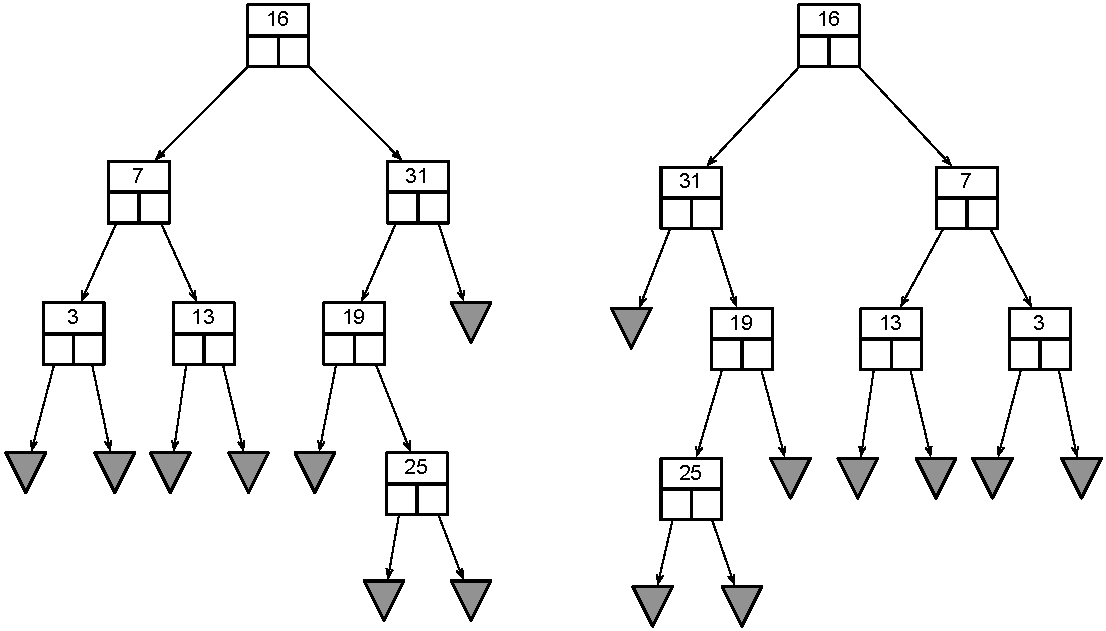
\includegraphics[scale=0.7]{images/binSearchTree_2}

\newpage

\item Implement a function \texttt{int comp(Tree t1, Tree t2)} that receives
two binary search trees, \texttt{t1} and \texttt{t2}, and returns 1 if they
are isomorphic, and 0 otherwise.

\vspace{6cm}

\item Implements a function \texttt{int* tree2Array(Tree t)}, which
receives a tree $t$, inserts all its elements into an array, and returns this
array.

\vspace{6cm}

\item Implement a function \texttt{int* treeSort(int* v, int n)}, which receives
an array \texttt{v} with \texttt{n} elements, and returns a new array, with
all the elements in \texttt{v} sorted in ascending order.
Your function must, necessarily, use a tree to sort the array.

\end{enumerate}

\end{enumerate}

\end{document}
